\documentclass[ignorenonframetext,]{beamer}
\setbeamertemplate{caption}[numbered]
\setbeamertemplate{caption label separator}{:}
\setbeamercolor{caption name}{fg=normal text.fg}
\usepackage{amssymb,amsmath}
\usepackage{ifxetex,ifluatex}
\usepackage{fixltx2e} % provides \textsubscript
\usepackage{lmodern}
\ifxetex
  \usepackage{fontspec,xltxtra,xunicode}
  \defaultfontfeatures{Mapping=tex-text,Scale=MatchLowercase}
  \newcommand{\euro}{€}
\else
  \ifluatex
    \usepackage{fontspec}
    \defaultfontfeatures{Mapping=tex-text,Scale=MatchLowercase}
    \newcommand{\euro}{€}
  \else
    \usepackage[T1]{fontenc}
    \usepackage[utf8]{inputenc}
      \fi
\fi



\geometry{paperwidth=200mm,paperheight=160mm}
\usetheme{Berlin}
\usecolortheme{beaver}

% use upquote if available, for straight quotes in verbatim environments
\IfFileExists{upquote.sty}{\usepackage{upquote}}{}
% use microtype if available
\IfFileExists{microtype.sty}{\usepackage{microtype}}{}
\usepackage{color}
\usepackage{fancyvrb}
\newcommand{\VerbBar}{|}
\newcommand{\VERB}{\Verb[commandchars=\\\{\}]}
\DefineVerbatimEnvironment{Highlighting}{Verbatim}{commandchars=\\\{\}}
% Add ',fontsize=\small' for more characters per line
\newenvironment{Shaded}{}{}
\newcommand{\KeywordTok}[1]{\textcolor[rgb]{0.00,0.44,0.13}{\textbf{{#1}}}}
\newcommand{\DataTypeTok}[1]{\textcolor[rgb]{0.56,0.13,0.00}{{#1}}}
\newcommand{\DecValTok}[1]{\textcolor[rgb]{0.25,0.63,0.44}{{#1}}}
\newcommand{\BaseNTok}[1]{\textcolor[rgb]{0.25,0.63,0.44}{{#1}}}
\newcommand{\FloatTok}[1]{\textcolor[rgb]{0.25,0.63,0.44}{{#1}}}
\newcommand{\CharTok}[1]{\textcolor[rgb]{0.25,0.44,0.63}{{#1}}}
\newcommand{\StringTok}[1]{\textcolor[rgb]{0.25,0.44,0.63}{{#1}}}
\newcommand{\CommentTok}[1]{\textcolor[rgb]{0.38,0.63,0.69}{\textit{{#1}}}}
\newcommand{\OtherTok}[1]{\textcolor[rgb]{0.00,0.44,0.13}{{#1}}}
\newcommand{\AlertTok}[1]{\textcolor[rgb]{1.00,0.00,0.00}{\textbf{{#1}}}}
\newcommand{\FunctionTok}[1]{\textcolor[rgb]{0.02,0.16,0.49}{{#1}}}
\newcommand{\RegionMarkerTok}[1]{{#1}}
\newcommand{\ErrorTok}[1]{\textcolor[rgb]{1.00,0.00,0.00}{\textbf{{#1}}}}
\newcommand{\NormalTok}[1]{{#1}}
\usepackage{graphicx}
\makeatletter
\def\maxwidth{\ifdim\Gin@nat@width>\linewidth\linewidth\else\Gin@nat@width\fi}
\def\maxheight{\ifdim\Gin@nat@height>\textheight0.8\textheight\else\Gin@nat@height\fi}
\makeatother
% Scale images if necessary, so that they will not overflow the page
% margins by default, and it is still possible to overwrite the defaults
% using explicit options in \includegraphics[width, height, ...]{}
\setkeys{Gin}{width=\maxwidth,height=\maxheight,keepaspectratio}

% Comment these out if you don't want a slide with just the
% part/section/subsection/subsubsection title:
\AtBeginPart{
  \let\insertpartnumber\relax
  \let\partname\relax
  \frame{\partpage}
}
\AtBeginSection{
  \let\insertsectionnumber\relax
  \let\sectionname\relax
  \frame{\sectionpage}
}
\AtBeginSubsection{
  \let\insertsubsectionnumber\relax
  \let\subsectionname\relax
  \frame{\subsectionpage}
}

\setlength{\parindent}{0pt}
\setlength{\parskip}{6pt plus 2pt minus 1pt}
\setlength{\emergencystretch}{3em}  % prevent overfull lines
\setcounter{secnumdepth}{0}

\title{Travelling Salesman Problem}
\author{Ignacio Cordón Castillo}
\institute{Doble Grado Matemáticas e Ingeniería Informática, Metaheurísticas, UGR}	

\begin{document}


\begin{frame}
\titlepage
\end{frame}

\begin{frame}[fragile]{Representación de soluciones}

Definimos una solución como un objeto \texttt{Route}, que almacena una
permutación de ciudades, una matriz de distancia, y contiene métodos de
cálculo del coste y de 2-opt de arcos y ciudades

\begin{Shaded}
\begin{Highlighting}[]
\KeywordTok{class} \NormalTok{Route:  }
    \KeywordTok{def} \OtherTok{__init__}\NormalTok{(}\OtherTok{self}\NormalTok{, permutation, dist):}
        \OtherTok{self}\NormalTok{.permutation = deepcopy(array(permutation))}
        \OtherTok{self}\NormalTok{.dist = array(dist)}
        \OtherTok{self}\NormalTok{.update_cost()}

    \KeywordTok{def} \NormalTok{update_cost(}\OtherTok{self}\NormalTok{):}
        \NormalTok{pairs = }\OtherTok{self}\NormalTok{.get_edges()}
        \OtherTok{self}\NormalTok{.cost = }\DataTypeTok{sum}\NormalTok{([}\OtherTok{self}\NormalTok{.dist[x,y] }\KeywordTok{for} \NormalTok{(x,y) in pairs])}

    \KeywordTok{def} \NormalTok{change_edges(}\OtherTok{self}\NormalTok{,i,j)}
        \NormalTok{i,j = }\DataTypeTok{min}\NormalTok{(i,j), }\DataTypeTok{max}\NormalTok{(i,j)}

        \NormalTok{rev = }\OtherTok{self}\NormalTok{.permutation[i:j]}
        \NormalTok{rev = rev[::-}\DecValTok{1}\NormalTok{]}
        \OtherTok{self}\NormalTok{.permutation[i:j] = rev}
        \OtherTok{self}\NormalTok{.update_cost()}

    \KeywordTok{def} \NormalTok{get_edges(}\OtherTok{self}\NormalTok{):}
        \NormalTok{shifted = append(}\OtherTok{self}\NormalTok{.permutation[}\DecValTok{1}\NormalTok{:], [}\OtherTok{self}\NormalTok{.permutation[}\DecValTok{0}\NormalTok{]])}
        \NormalTok{pairs = }\DataTypeTok{zip}\NormalTok{(}\OtherTok{self}\NormalTok{.permutation, shifted)}
        \KeywordTok{return}\NormalTok{(pairs)}
            
\end{Highlighting}
\end{Shaded}

\end{frame}

\begin{frame}{Simulated Annealing}

Emplea esquema de enfriamiento geométrico, con operador de generación de
vecino 2-opt de arcos, y selección de temperatura inicial a:

\[T_0 = \frac{\mu}{-log(\phi)} \cdot Cost(S_0)  \]

\begin{itemize}
\item
  \textbf{\texttt{n\_iter}}: Número de evaluaciones que se hacen de la
  función objetivo
\item
  \textbf{\texttt{max\_exitos}}: Número de máximo de mejoras encontradas
  en un vecindario
\item
  \textbf{\texttt{max\_vecinos}}: Número de vecinos que se generarán en
  cada exploración de vecindario
\item
  \textbf{\texttt{alpha}}: factor de descenso de la media geométrica
  $T_k = \alpha \cdot T_{k-1}$
\item
  \textbf{\texttt{mu}}
\item
  \textbf{\texttt{phi}}
\end{itemize}

\end{frame}

\begin{frame}[fragile]{Simulated Annealing}

\begin{Shaded}
\begin{Highlighting}[]
\KeywordTok{def} \NormalTok{simulated_annealing(}\OtherTok{self}\NormalTok{, max_iter, max_exitos, max_vecinos, alpha, mu, phi):}
        
    \KeywordTok{while} \NormalTok{num_iter < max_iter:           }
        \KeywordTok{while} \NormalTok{num_iter < max_iter and num_vecinos < max_vecinos and exitos < max_exitos:}

            \NormalTok{candidate = deepcopy(solution)}
            \NormalTok{u = randint(}\DecValTok{0}\NormalTok{, n)}
            \NormalTok{v = randint(}\DecValTok{0}\NormalTok{, n)   }
            \NormalTok{candidate.change_edges(u,v)}

            \NormalTok{diff_cost = candidate.cost - solution.cost}

            \KeywordTok{if} \NormalTok{(diff_cost < }\DecValTok{0} \NormalTok{or random() < exp(-diff_cost*}\FloatTok{1.0}\NormalTok{/t)):}
                \NormalTok{solution = deepcopy(candidate)}
                \NormalTok{exitos+=}\DecValTok{1}

                \KeywordTok{if} \NormalTok{(solution.cost < best_solution.cost):}
                    \NormalTok{best_solution = deepcopy(solution)}

            \NormalTok{num_iter+=}\DecValTok{1}
            \NormalTok{num_vecinos+=}\DecValTok{1}

        \NormalTok{t = alpha*t}

    \KeywordTok{return} \NormalTok{best_solution}
    
\end{Highlighting}
\end{Shaded}

\end{frame}

\begin{frame}{Tabu Search}

Emplea memoria de corto y largo plazo, y operador de vecino 2-opt de
arcos.

La memoria de largo plazo \textbf{\texttt{edge\_freq}} es una matriz que
almacena las veces que un arco \texttt{(p,q)} ha salido en un vecino
bueno del vecindario (uno que mejorase al mejor hasta el momento
\textbf{\texttt{best\_neighbour}}).

Cuando se produce la reinicialización (con probabilidad
\textbf{\texttt{1-prob\_intensificacion}} cada vez que se alcanza
\textbf{\texttt{limit\_restart}} de vecinos sin elementos tabú que no
mejoran a \textbf{\texttt{best\_neighbour}}), se resetean todos los
valores de la memoria de largo plazo a 0.

La intensificación reinicia la búsqueda a la mejor solución encontrada
\textbf{\texttt{best\_solution}} con una probabilidad de
\textbf{\texttt{prob\_intensificacion}} cada vez que se llega un número
\textbf{\texttt{limit\_restart}} de vecinos sin elementos tabú que no
mejoran a \textbf{\texttt{best\_neighbour}}.

\begin{itemize}
\item
  \textbf{\texttt{max\_iter}}: Número de vecinos que se generan
\item
  \textbf{\texttt{max\_vecinos}}: Número de vecinos que se generarán en
  cada exploración de vecindario
\item
  \textbf{\texttt{limit\_restart}}: Número de evaluaciones de la función
  objetivo que no han mejorado
\item
  \textbf{\texttt{tabu\_tenencia}}: Tamaño de la
  \textbf{\texttt{tabu\_list}} que contiene los movimientos 2-opt más
  recientes
\item
  \textbf{\texttt{aspiration\_tol}}: Criterio de aspiración. Da la
  tolerancia en coste en el intervalo $[0,1]$ frente a la mejor solución
  obtenida hasta el momento
\item
  \textbf{\texttt{prob\_intensificacion}}: Probabilidad con la que tras
  un número \textbf{\texttt{limit\_restart}} de vecinos que no mejoran,
  se intensificará la búsqueda sobre la mejor solución hasta el momento.
\end{itemize}

\end{frame}

\begin{frame}[fragile]{Tabu Search}

\begin{block}{Reinicialización e intensificación}

\begin{Shaded}
\begin{Highlighting}[]

\KeywordTok{def} \NormalTok{_make_permutation(}\OtherTok{self}\NormalTok{, edge_freq):}
    \NormalTok{edge_freq = array(edge_freq)}
    \NormalTok{n = }\DataTypeTok{len}\NormalTok{(edge_freq)}
    \NormalTok{permutation = array([}\DecValTok{0}\NormalTok{]*n)}
    \NormalTok{visited = array([}\OtherTok{True}\NormalTok{] + [}\OtherTok{False}\NormalTok{]*(n}\DecValTok{-1}\NormalTok{))}

    \KeywordTok{for} \NormalTok{i in }\DataTypeTok{range}\NormalTok{(}\DecValTok{1}\NormalTok{,n):}
        \NormalTok{min_freq = }\DataTypeTok{float}\NormalTok{(}\StringTok{"inf"}\NormalTok{)}

        \KeywordTok{for} \NormalTok{j in where(visited == }\OtherTok{False}\NormalTok{)[}\DecValTok{0}\NormalTok{]:}
            \KeywordTok{if} \NormalTok{edge_freq[ permutation[i}\DecValTok{-1}\NormalTok{],j ] < min_freq:}
                \NormalTok{min_freq = edge_freq[ permutation[i}\DecValTok{-1}\NormalTok{],j ]}
                \NormalTok{selected = j}

        \NormalTok{visited[selected] = }\OtherTok{True}
        \NormalTok{permutation[i] = selected}

    \KeywordTok{return} \NormalTok{permutation}
\end{Highlighting}
\end{Shaded}

\end{block}

\end{frame}

\begin{frame}[fragile]{Tabu Search}

\begin{block}{Reinicialización e intensificación}

\begin{Shaded}
\begin{Highlighting}[]
\KeywordTok{def} \NormalTok{tabu_search(}\OtherTok{self}\NormalTok{, max_iter, max_vecinos, limit_restart, }
                \NormalTok{tabu_tenencia, aspiration_tol, prob_intensificacion):}

    \KeywordTok{while} \NormalTok{i < max_iter:                }
        \NormalTok{j = }\DecValTok{0}

        \KeywordTok{if} \NormalTok{restart:}
            \NormalTok{u = random()}

            \KeywordTok{if} \NormalTok{(u < prob_intensificacion):}
                \NormalTok{neighbour = deepcopy(best_solution)}
            \KeywordTok{else}\NormalTok{: }
                \NormalTok{neighbour = Route(}\OtherTok{self}\NormalTok{._make_permutation(edge_freq), }\OtherTok{self}\NormalTok{.dist)}
                \NormalTok{edge_freq = array([[}\DecValTok{0}\NormalTok{]*n]*n)}

            \NormalTok{restart = }\OtherTok{False}
            \NormalTok{non_improving = }\DecValTok{0}                    

        \NormalTok{best_neighbour = deepcopy(neighbour)}
        \NormalTok{u_tabu, v_tabu = }\OtherTok{None}\NormalTok{, }\OtherTok{None}
\end{Highlighting}
\end{Shaded}

\end{block}

\end{frame}

\begin{frame}[fragile]{Tabu Search}

\begin{block}{Exploración del entorno y gestión de la lista tabú}

\begin{Shaded}
\begin{Highlighting}[]
        \KeywordTok{while} \NormalTok{i < max_iter and j < max_vecinos and not restart:  }
            \CommentTok{# Generamos los índices de los arcos a cambiar}
            \NormalTok{candidate = deepcopy(neighbour)    }
            \NormalTok{u = randint(}\DecValTok{0}\NormalTok{, n)}
            \NormalTok{v = randint(}\DecValTok{0}\NormalTok{, n)   }
            \NormalTok{candidate.change_edges(u,v)}

            \NormalTok{eval_solution = }\OtherTok{True}

            \KeywordTok{for} \NormalTok{(p,q) in candidate.get_edges():}
                \NormalTok{edge_freq[p,q] += }\DecValTok{1}\NormalTok{;}
                \NormalTok{edge_freq[q,p] += }\DecValTok{1}

            \CommentTok{# Si hay arcos comunes entre ambos}
            \KeywordTok{if} \NormalTok{(}\DataTypeTok{set}\NormalTok{([(u,v)]) & }\DataTypeTok{set}\NormalTok{(tabu_list)):}
                \NormalTok{eval_solution = }\OtherTok{False}

                \CommentTok{"""Criterio de aspiración"""}
                \KeywordTok{if} \NormalTok{candidate.cost < aspiration_tol*best_solution.cost:}
                    \NormalTok{eval_solution = }\OtherTok{True}
\end{Highlighting}
\end{Shaded}

\end{block}

\end{frame}

\begin{frame}[fragile]{Tabu Search}

\begin{block}{Exploración del entorno y gestión de la lista tabú}

\begin{Shaded}
\begin{Highlighting}[]
            \KeywordTok{if} \NormalTok{eval_solution:                                       }
                \KeywordTok{if} \NormalTok{candidate.cost < best_neighbour.cost:}
                    \NormalTok{best_neighbour = deepcopy(candidate)}
                    \NormalTok{u_tabu, v_tabu = u,v     }

                    \KeywordTok{if} \NormalTok{candidate.cost < best_solution.cost:}
                        \NormalTok{best_solution = deepcopy(candidate)                      }
                        \NormalTok{improvement = }\OtherTok{True}
                \KeywordTok{else}\NormalTok{:}
                    \NormalTok{non_improving += }\DecValTok{1}
                    \NormalTok{restart = (non_improving == limit_restart)          }

            \NormalTok{j+=}\DecValTok{1}
            \NormalTok{i+=}\DecValTok{1}
        \CommentTok{"""Fin de exploración del vecindario"""}

        \NormalTok{neighbour = deepcopy(best_neighbour)}
        \CommentTok{# Arcos del mejor vecino}
        \KeywordTok{if} \NormalTok{u_tabu is not }\OtherTok{None}\NormalTok{:}
            \NormalTok{tabu_list[ }\DataTypeTok{next}\NormalTok{(index) ] = (u_tabu, v_tabu)}
        \KeywordTok{else}\NormalTok{:}
            \NormalTok{tabu_list[ }\DataTypeTok{next}\NormalTok{(index) ] = }\OtherTok{None}

    \CommentTok{"""Fin de toda la exploración"""}
    \KeywordTok{return} \NormalTok{best_solution}
\end{Highlighting}
\end{Shaded}

\end{block}

\end{frame}

\begin{frame}{Simulated Annealing}

\begin{block}{Parámetros empleados}

\begin{itemize}
\item
  \textbf{\texttt{n\_iter}}: El número de iteraciones se fija en cien
  veces el tamaño del problema ($n$, número de ciudades)
\item
  \textbf{\texttt{max\_vecinos}}: 10 $\cdot n$
\item
  \textbf{\texttt{max\_exitos}}: 0.1 $\cdot n$
\item
  \textbf{\texttt{alpha}}: 0.95
\item
  \textbf{\texttt{mu}}: 0.1
\item
  \textbf{\texttt{phi}}: 0.1
\end{itemize}

\end{block}

\end{frame}

\begin{frame}{Simulated Annealing}

\begin{block}{eil101}

\begin{itemize}
\item
  Media ejecuciones: 752.95
\item
  Mejor ejecución: 743.97
\item
  Óptimo: 629
\end{itemize}

\begin{figure}[htbp]
\centering
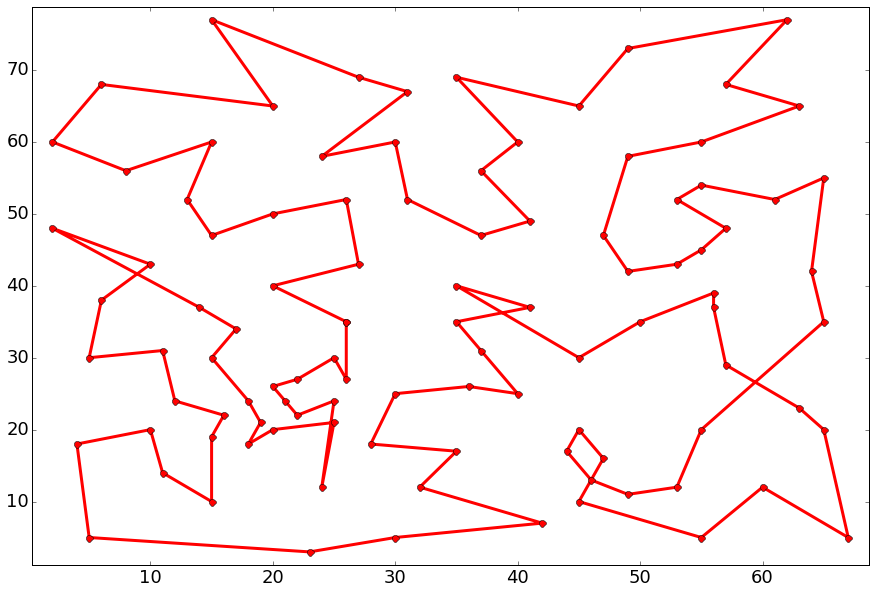
\includegraphics[width=0.8\textwidth]{./images/eil101sa.png}
\end{figure}

\end{block}

\end{frame}

\begin{frame}{Simulated Annealing}

\begin{block}{berlin52}

\begin{itemize}
\item
  Media ejecuciones: 8593.93
\item
  Mejor ejecución: 8383.45
\item
  Óptimo: 7542
\end{itemize}

\begin{figure}[htbp]
\centering
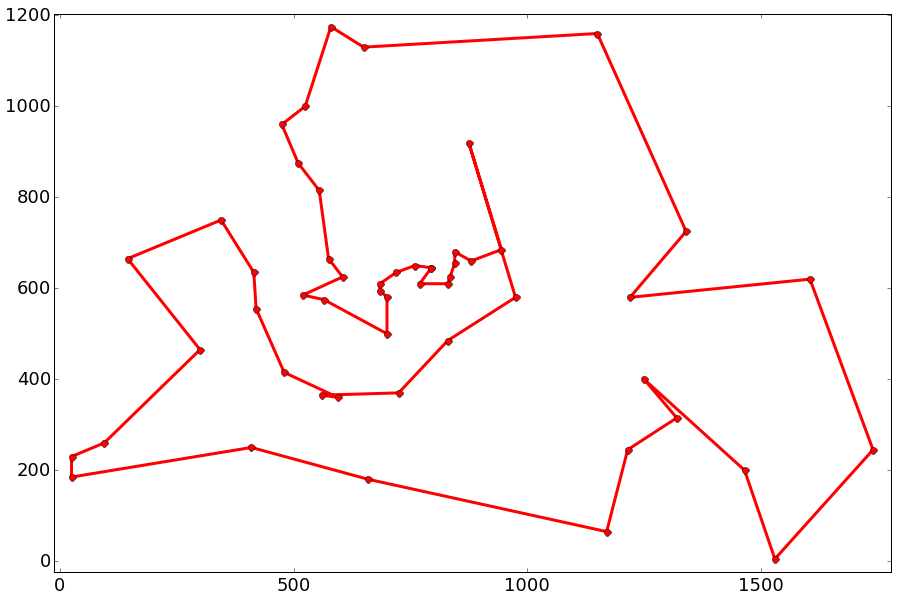
\includegraphics[width=0.8\textwidth]{./images/berlin52sa.png}
\end{figure}

\end{block}

\end{frame}

\begin{frame}{Simulated Annealing}

\begin{block}{ch150}

\begin{itemize}
\item
  Media ejecuciones: 9162.65
\item
  Mejor ejecución: 8365.03
\item
  Óptimo: 6528
\end{itemize}

\begin{figure}[htbp]
\centering
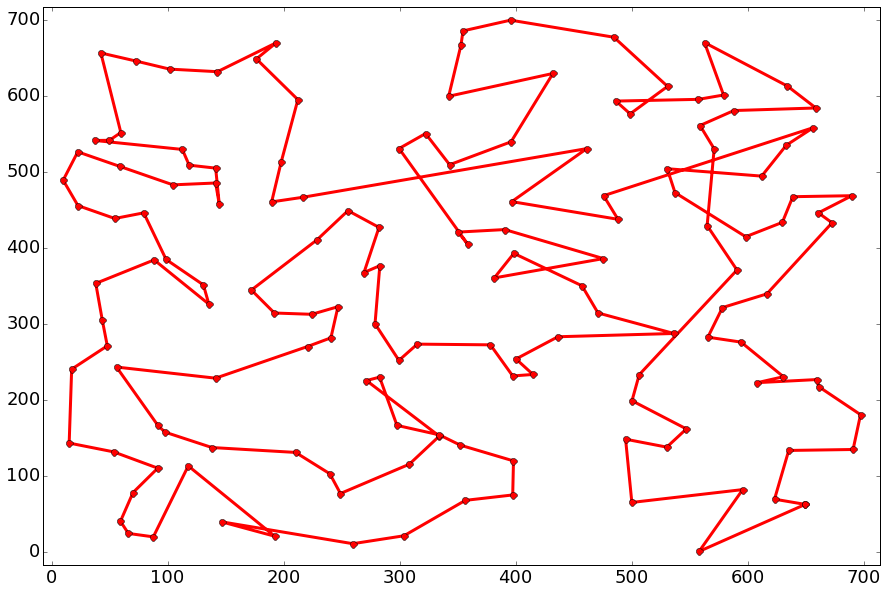
\includegraphics[width=0.8\textwidth]{./images/ch150sa.png}
\end{figure}

\end{block}

\end{frame}

\begin{frame}{Simulated Annealing}

\begin{block}{d198}

\begin{itemize}
\item
  Media ejecuciones: 22258.84
\item
  Mejor ejecución: 21293.31
\item
  Óptimo: 15780
\end{itemize}

\begin{figure}[htbp]
\centering
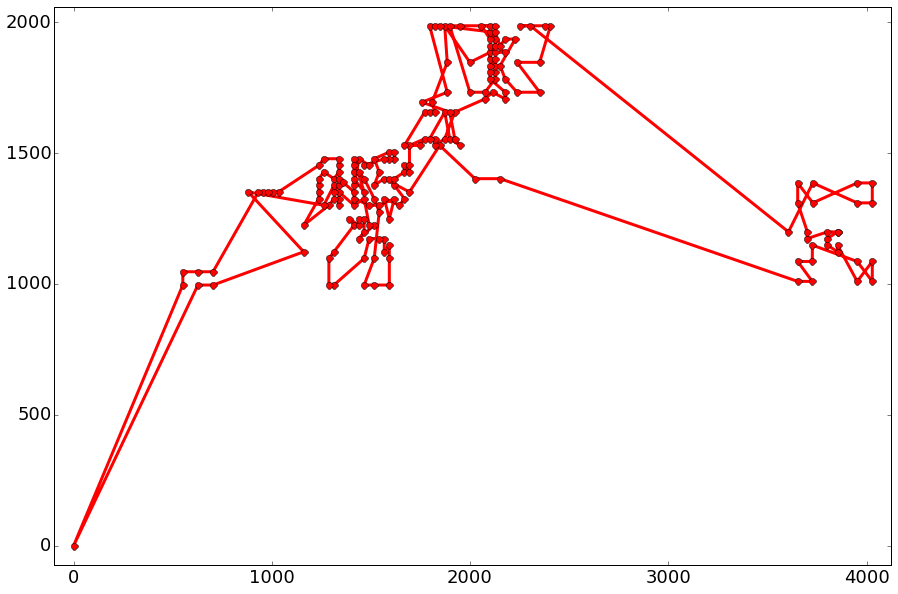
\includegraphics[width=0.8\textwidth]{./images/d198sa.png}
\end{figure}

\end{block}

\end{frame}

\begin{frame}{Simulated Annealing}

\begin{block}{rd400}

\begin{itemize}
\item
  Media ejecuciones: 30425.56
\item
  Mejor ejecución: 29360.85
\item
  Óptimo: 15281
\end{itemize}

\begin{figure}[htbp]
\centering
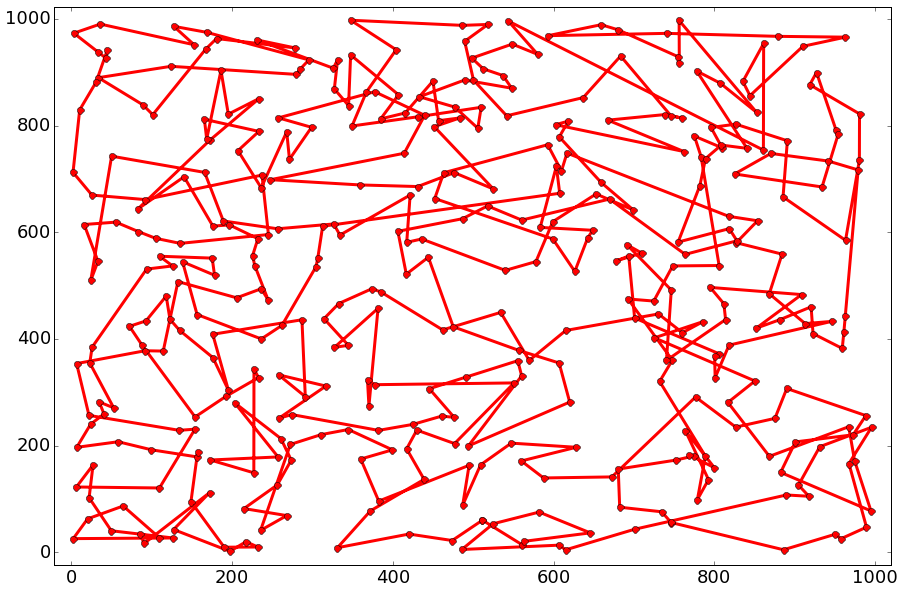
\includegraphics[width=0.8\textwidth]{./images/rd400sa.png}
\end{figure}

\end{block}

\end{frame}

\begin{frame}{Tabu Search}

\begin{block}{Parámetros empleados}

\begin{itemize}
\item
  \textbf{\texttt{n\_iter}}: El número de iteraciones se fija en cien
  veces el tamaño del problema ($n$, número de ciudades)
\item
  \textbf{\texttt{max\_vecinos}}: 25
\item
  \textbf{\texttt{limit\_restart}}: 25
\item
  \textbf{\texttt{tabu\_tenencia}}: El tamaño de la tenencia se fija en
  el doble de $n$, número de ciudades del problema
\item
  \textbf{\texttt{aspiration\_tol}}: 1
\item
  \textbf{\texttt{prob\_intensificacion}}: 0.95
\end{itemize}

\end{block}

\end{frame}

\begin{frame}{Tabu Search}

\begin{block}{eil101}

\begin{itemize}
\item
  Media ejecuciones: 778.41
\item
  Mejor ejecución: 748.15
\item
  Óptimo: 629
\end{itemize}

\begin{figure}[htbp]
\centering
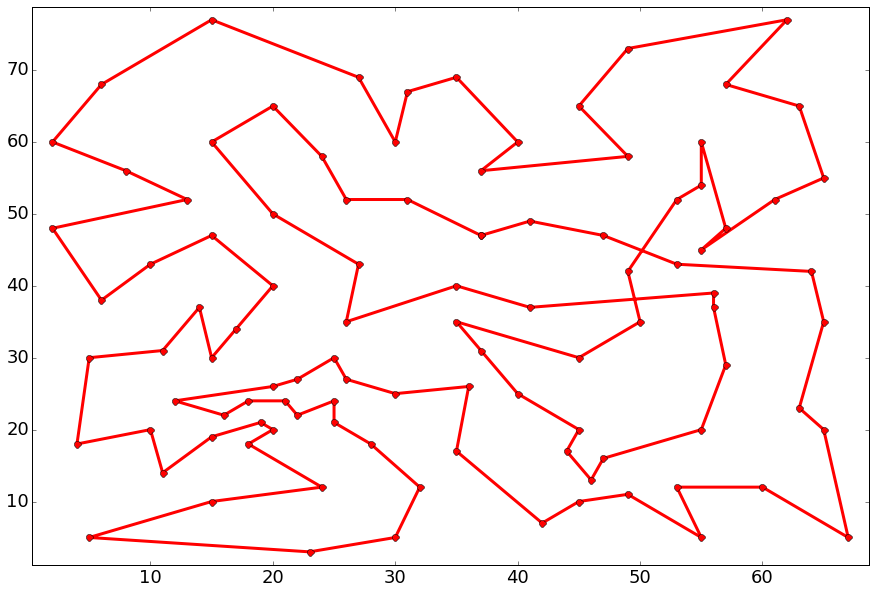
\includegraphics[width=0.8\textwidth]{./images/eil101ts.png}
\end{figure}

\end{block}

\end{frame}

\begin{frame}{Tabu Search}

\begin{block}{berlin52}

\begin{itemize}
\item
  Media ejecuciones: 8526.00
\item
  Mejor ejecución: 8076.46
\item
  Óptimo: 7542
\end{itemize}

\begin{figure}[htbp]
\centering
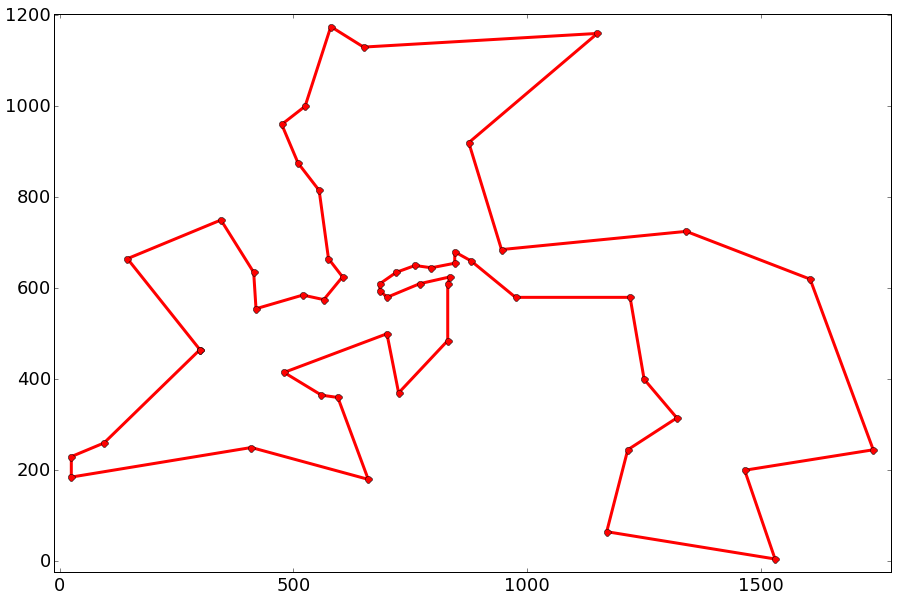
\includegraphics[width=0.8\textwidth]{./images/berlin52ts.png}
\end{figure}

\end{block}

\end{frame}

\begin{frame}{Tabu Search}

\begin{block}{ch150}

\begin{itemize}
\item
  Media ejecuciones: 9641.97
\item
  Mejor ejecución: 9606.00
\item
  Óptimo: 6528
\end{itemize}

\begin{figure}[htbp]
\centering
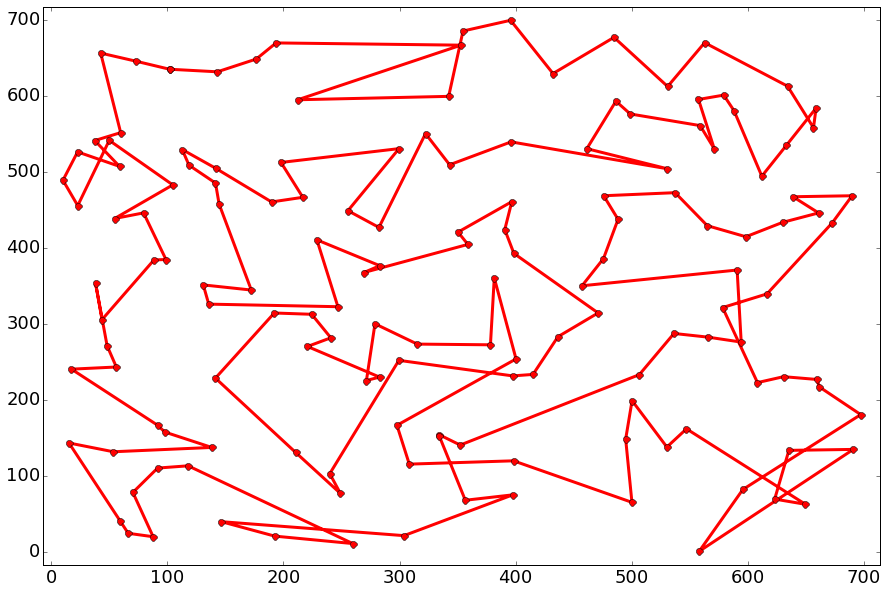
\includegraphics[width=0.8\textwidth]{./images/ch150ts.png}
\end{figure}

\end{block}

\end{frame}

\begin{frame}{Tabu Search}

\begin{block}{d198}

\begin{itemize}
\item
  Media ejecuciones: 19275.58
\item
  Mejor ejecución: 18426.83
\item
  Óptimo: 15780
\end{itemize}

\begin{figure}[htbp]
\centering
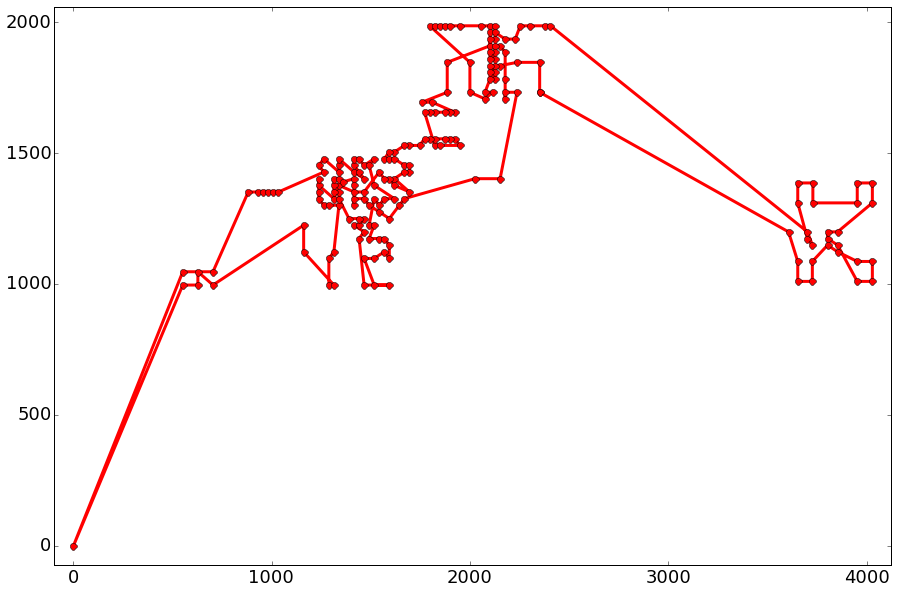
\includegraphics[width=0.8\textwidth]{./images/d198ts.png}
\end{figure}

\end{block}

\end{frame}

\begin{frame}{Tabu Search}

\begin{block}{rd400}

\begin{itemize}
\item
  Media ejecuciones: 32433.59
\item
  Mejor ejecución: 31790.21
\item
  Óptimo: 15281
\end{itemize}

\begin{figure}[htbp]
\centering
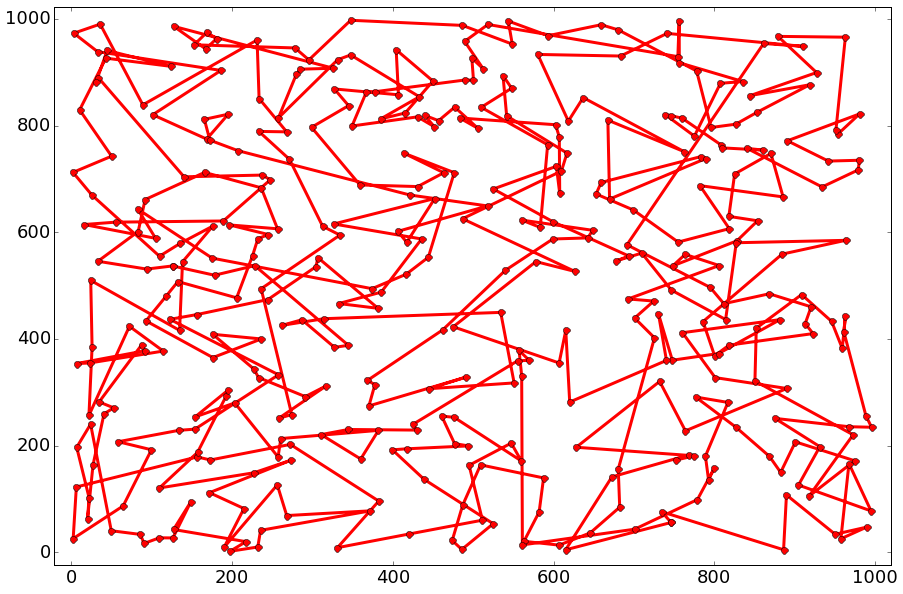
\includegraphics[width=0.8\textwidth]{./images/rd400ts.png}
\end{figure}

\end{block}

\end{frame}

\end{document}
